\documentclass[10pt]{article}

% ---------------------------------------------------------------------------
% S&P 500 cross-sectional relative-return case study.
% Compile: pdflatex sp500_case_study.tex  (run twice for references).
% Figures live in report/figures/*.pdf, generated by scripts/make_report_figures.py
% ---------------------------------------------------------------------------

\usepackage[margin=0.78in]{geometry}
\usepackage{booktabs}
\usepackage{graphicx}
\usepackage{amsmath}
\usepackage{microtype}
\usepackage{enumitem}
\usepackage[hidelinks]{hyperref}
\usepackage{caption}
\usepackage{float}
\captionsetup{font=small,labelfont=bf}
\setlist{nosep,leftmargin=1.4em}
\graphicspath{{figures/}}

\setlength{\parskip}{0.22em}
\setlength{\parindent}{0pt}

\title{\vspace{-2.5em}Predicting Cross-Sectional Relative Returns in the S\&P~500:\\
A Feature-Engineering and Walk-Forward Modeling Case Study}
\author{Quantitative Research Case Study}
\date{}

\begin{document}
\maketitle
\vspace{-3em}

% ===========================================================================
\section{Problem and Approach}
% ===========================================================================

The task is to predict \emph{relative} future stock returns inside the S\&P~500:
not whether the market goes up, but which stocks will out- or under-perform
their peers. This framing is deliberate. Index-level direction is dominated by
macro factors that daily OHLCV data cannot forecast, whereas the
\emph{cross-section} of returns carries persistent, tradable structure
(momentum, reversal, liquidity, volatility, and sector-rotation effects) that is
learnable from price and volume alone.

We therefore predict each stock's forward return \emph{in excess of its market
and sector}, convert model predictions into a validation-selected ensemble
score, and then use that score in explicitly specified portfolio tests. The
primary trading evaluation is a cost-adjusted, sector-neutral decile long--short
portfolio: within each sector, long the top-scored stocks and short the
bottom-scored stocks, then combine sectors into a dollar-neutral book. The
entire pipeline is built to be honest about look-ahead leakage, overlapping-window
inflation, transaction costs, and survivorship bias, because in this problem the
easiest way to produce a spectacular-looking result is to make a methodological
mistake.

\textbf{Headline design.} Curated technical/liquidity/cross-sectional features
$\rightarrow$ sector- and market-relative forward-return targets $\rightarrow$ a
single-factor momentum baseline, Ridge, LightGBM, XGBoost, MLP, and supervised
relation-aware graph variants $\rightarrow$ validation-selected cross-sectional
rank ensembles $\rightarrow$ rank IC / ICIR, regime stability, and
transaction-cost-aware portfolio backtests. The headline horizon is the
5-trading-day relative return, with the 10-trading-day sector-neutral portfolio
used as the main risk-adjusted robustness case.

% ===========================================================================
\section{Data}
% ===========================================================================

We use only two files: \texttt{sp500\_stocks.csv} (daily OHLCV per ticker) and
\texttt{sp500\_companies.csv} (sector, sub-industry, headquarters, founding year,
and index \texttt{date\_added}). No fundamentals, analyst, macro, or external
listing data are used. The cleaned panel covers 503 symbols from 2000-01 to
2026-06 (2.926M stock-day rows).

\textbf{Price adjustment (data quality).} The raw file exposes only a
\texttt{close} column and no separate \texttt{adj\_close}. We therefore audited
major split events and verified that this \texttt{close} behaves as an adjusted
close price: around NVDA's 2024-06-10 10:1 split (120.68 $\rightarrow$ 121.58)
and AAPL's 2020-08-31 4:1 split (121.06 $\rightarrow$ 125.17) there is no
split-day gap, consistent with a \texttt{yfinance auto\_adjust=True} export. In
this study, \texttt{close} is therefore treated as the adjusted close used for
all returns, momentum, volatility, and forward-return targets. Residual
uncertainty about dividend adjustment is treated as a minor data-quality caveat.

\textbf{Raw cleaning.} The CSV-to-Parquet preparation step normalizes ticker
strings, enforces one row per \texttt{symbol,date}, drops rows with missing core
OHLCV fields, non-positive prices or volume, and impossible OHLC relationships
(\texttt{high} below open/low/close or \texttt{low} above open/high/close). The
raw stock file has no core missing values or duplicate stock-days, but it does
contain 4,413 zero-volume rows and one OHLC inversion; these 4,414 rows are
removed before feature construction. Large but plausible moves are audited rather
than deleted: 44 stock-days have absolute one-day returns above 50\%, while none
exceed the 300\% hard error threshold. Company metadata are also normalized and
deduplicated; all 503 tickers have sector and sub-industry labels.

\textbf{Survivorship bias.} The constituent list is effectively the
\emph{current} membership applied to history, so firms that went bankrupt, were
delisted, or were acquired (Enron, Lehman, Bear Stearns, WaMu, Sears, Kodak,
Yahoo, Celgene, Xilinx, \dots) are absent. This biases backtests optimistically
and is discussed quantitatively in \S\ref{sec:discussion}. We do not claim to
correct it; we bound its impact and avoid designs that amplify it.

% ===========================================================================
\section{Feature Engineering}
% ===========================================================================

Each row is one stock-day observation, and every feature uses only information
available at or before that date (all rolling windows are backward-looking with
an explicit \texttt{shift}). We build $\approx$500 features in economically
motivated groups:

\begin{itemize}
  \item \textbf{Price / momentum / reversal:} multi-horizon returns
  (1--252d), log returns, skip-window momentum, momentum acceleration,
  short-term reversal, intraday/overnight decomposition, close-in-bar location.
  \emph{Captures short-term reversal and medium-term momentum.}
  \item \textbf{Volatility / tail / drawdown:} rolling, upside/downside,
  Parkinson and Garman--Klass volatility, ATR, skew/kurtosis, drawdown from
  recent highs. \emph{Controls for risk state and crash sensitivity.}
  \item \textbf{Trend / technical:} SMA/EMA gaps and slopes, MACD, RSI,
  Bollinger z-score/bandwidth/\%b, channel position, breakout distance,
  Williams~\%R, CCI. \emph{Encodes overbought/oversold and trend regimes.}
  \item \textbf{Liquidity / volume:} log dollar volume, volume z-scores and
  momentum, Amihud illiquidity, return-per-dollar-volume. \emph{Captures
  attention, liquidity shocks, and transaction-cost pressure.}
  \item \textbf{Market regime:} equal-weight market return, breadth,
  cross-sectional dispersion, market volatility. \emph{Relative-return
  predictability is regime-dependent.}
  \item \textbf{Statistical linkage / residual risk:} rolling market beta,
  market correlation, idiosyncratic return, and idiosyncratic volatility.
  \emph{Captures stock-level residual behavior after market exposure is
  removed.}
  \item \textbf{Sector / sub-industry and peer / style / geography:} group
  returns, breadth, dispersion, leave-one-out peer means, headquarters-region
  peers, and style buckets. \emph{Separates stock-specific alpha from group
  movement.}
  \item \textbf{Graph relation features:} two graph feature families are kept
  separate. The original \texttt{fixed\_graph} variant uses deterministic
  same-sector/sub-industry, style-nearest-neighbor, and rolling-correlation graph
  relation embeddings. The \texttt{supervised\_graph} variant uses out-of-fold
  supervised GAT embeddings and scores. \emph{This separates static peer-structure
  features from supervised relation-aware graph learning.}
  \item \textbf{Cross-sectional transforms:} date-wise z-scores/ranks plus
  sector- and sub-industry-neutral versions of the key signals.
  \emph{Because the target is relative, cross-sectional normalization is usually
  more informative than raw levels.}
\end{itemize}

\textbf{Feature audit and sanity check.} The rebuilt feature manifest contains
525 non-target columns and 40 target columns. The large count is not 525
independent ideas; it comes from expanding a smaller set of economic signals
across lookback windows, related definitions, and neutralization transforms.
For example, the cross-sectional layer alone contributes 168 columns by applying
date-wise, sector-wise, and sub-industry-wise z-scores and ranks to selected
base signals. The default walk-forward models do not use the full catalog:
they use a curated 61-column \texttt{core} set covering momentum/reversal,
volatility, technical indicators, liquidity, market/industry context, and key
  cross-sectional ranks. The executable grid treats graph inclusion as a feature
  variant: \texttt{tabular} uses those 61 core features, while
  \texttt{fixed\_graph} (called \texttt{graph} in some lower-level pipeline
  outputs) appends 19 deterministic graph columns
(\texttt{graph\_emb\_0}--\texttt{graph\_emb\_15}
plus relation-fusion weights for sector, style kNN, and rolling correlation).
The three relation weights
(\texttt{graph\_rel\_weight\_sector},
\texttt{graph\_rel\_weight\_style\_knn}, and
\texttt{graph\_rel\_weight\_rolling\_corr}) are normalized across relations and
therefore sum to about one up to floating-point error; for each stock-date they
  indicate whether the graph relation embedding relies more on sector peers,
  style-nearest peers, or rolling-correlation peers. Separately,
  \texttt{supervised\_graph} appends target-matched out-of-fold GAT score,
  embedding, and relation-weight columns, while \texttt{graph\_supervised} is the
  combined fixed-graph plus supervised-GAT variant. All variants use the same
  targets, folds, models, costs, purge/embargo, and hold-out protocol.

We explicitly verified that the expected factor families are present:
12-minus-1-month momentum (\texttt{mom\_252d\_skip\_21d}), short-term reversal
(\texttt{rev\_*}), volatility/range estimators, Bollinger features,
\texttt{MACD}, RSI-style oscillators, Amihud illiquidity, and
date/sector/sub-industry z-score and rank transforms. The short-cycle feature
block also includes the signals most likely to be orthogonal to 12--1 momentum:
1--5 day reversal, Amihud liquidity/impact, volume shocks, market breadth,
cross-sectional dispersion, and rolling idiosyncratic return after market-beta
removal. As a usefulness check, we
ran a single-factor daily rank-IC scan on the cleaned 2008--2026 panel using the
same T+1 label shift, bottom-10\% liquidity filter, and 1\%/99\% within-date
winsorization as the modeling pipeline. Table~\ref{tab:feature_sanity} shows the
largest effects in the core set. The magnitudes are small, as expected for daily
cross-sectional equity alpha, but the signs are economically coherent: short-term
overextension tends to reverse, 12--1 momentum is positive, and liquidity/impact
variables contain weak but measurable information.

\begin{table}[t]
  \centering
  \caption{Single-factor sanity check on core features, target
  \texttt{target\_excess\_sector\_fwd\_5d}. Mean IC is the average daily
  Spearman rank correlation after the production cleaning/evaluation controls.}
  \label{tab:feature_sanity}
  \small
  \begin{tabular}{lrl}
    \toprule
    Feature & Mean IC & Interpretation \\
    \midrule
    \texttt{sector\_rank\_sma\_gap\_20d} & -0.0131 & within-sector short-term reversal \\
    \texttt{ret\_5d} & -0.0125 & recent winners partially mean-revert \\
    \texttt{amihud\_20d} & +0.0123 & liquidity / price-impact information \\
    \texttt{log\_dollar\_volume} & -0.0123 & liquidity/size relation in relative returns \\
    \texttt{mom\_252d\_skip\_21d} & +0.0102 & 12--1 month momentum survives weakly \\
    \texttt{rsi\_14d} & -0.0099 & overbought names tend to cool off \\
    \bottomrule
  \end{tabular}
\end{table}

\textbf{Prediction target.} For horizon $h$ we define the forward total return
$r^{(h)}_{i,t}$ and subtract a contemporaneous group mean to obtain
sector/market-relative targets, e.g.
$\text{target\_excess\_sector\_fwd\_}h\text{d}_{i,t} = r^{(h)}_{i,t} -
\overline{r}^{(h)}_{\text{sector}(i),t}$. Targets are forward-looking and are
strictly excluded from the feature matrix. The target generator also writes a
date-wise percentile-rank target, \texttt{target\_rank\_fwd\_}h\texttt{d}, so
short-horizon experiments can use volatility-normalized, ranked, or winsorized
labels when raw returns are too noisy. The implemented horizon grid covers
$h\in\{1,5,10,20,30,40,50,60,70,80,90\}$; this report emphasizes 5d for the
main rank test and 10d for the sector-neutral risk-adjusted portfolio test.

\textbf{Execution timing.} The raw target columns are generated on each feature
date, but the model is evaluated with a one-day implementation lag. A feature row
at date $t$ is interpreted as information available after the $t$ close; the
signal is therefore tradeable only from $t{+}1$. In code, the effective training
label is the raw target shifted one trading day forward, so a row dated $t$ is
matched to the forward return window that starts from the next trading day. This
is the convention used for both rank-IC evaluation and portfolio PnL.

% ===========================================================================
\section{Methodology}
% ===========================================================================

\subsection{Models}
We compare, from simple to flexible:
(i) a \textbf{single-factor momentum} baseline (rank by 12-minus-1-month
momentum); (ii) \textbf{Ridge} regression (linear, strong regularization);
(iii) \textbf{LightGBM} and (iv) \textbf{XGBoost} gradient-boosted trees
(non-linear, interaction-aware); and (v) a small \textbf{PyTorch MLP}
(two hidden layers, dropout, weight decay, early stopping on validation). The
MLP is kept deliberately small and is \emph{not} tuned until it wins;
\S\ref{sec:results} reports its honest standing --- competitive on in-sample
validation IC, but not stable enough to headline once the untouched hold-out,
turnover, and momentum benchmark are applied.

\textbf{Momentum-residual overlay.} Because the single-factor momentum baseline
is strong, the implemented post-training evaluator does not force ML to replace
momentum. For each date, both the baseline score and model score are converted
to cross-sectional z-scores, the model score is residualized on the momentum
score, and the final overlay signal is
\[
  s_{i,t}=z(\text{momentum}_{i,t})+\lambda z(\widehat{\varepsilon}_{i,t}),
\]
where $\widehat{\varepsilon}_{i,t}$ is the model component orthogonal to
momentum within that day's cross-section. The grid evaluates
$\lambda\in\{0,0.25,0.5,0.75,1,1.5\}$, with $\lambda{=}0$ reproducing the
momentum baseline. The overlay is selected on validation ICIR and net portfolio
metrics only, so the test split is not used to tune the amount of residual ML
alpha.

\textbf{Graph feature variants.} Graph features are predictive inputs, not
separate trading rules. The \texttt{fixed\_graph} variant is the original
deterministic graph embedding: it builds sector, style-nearest-neighbor, and
rolling-correlation relations from information available at the feature date and
feeds the resulting \texttt{graph\_emb\_*} and relation-weight columns into the
same tabular models. The \texttt{supervised\_graph} variant is the GAT
extension: a supervised GAT is trained on the same time splits, then emits an
out-of-fold \texttt{supervised\_graph\_score}, relation weights, and
low-dimensional embeddings. The optional \texttt{graph\_supervised} variant
combines both feature families. All graph variants are evaluated under the same
purge, embargo, execution-lag, validation, cost, and portfolio rules as the
tabular variant.

\begin{table}[H]
  \centering
  \caption{Graph feature variants used in the model grid. The table separates
  deterministic graph embeddings from supervised GAT embeddings before any
  portfolio construction is applied.}\label{tab:graph_variants}
  \scriptsize
  \setlength{\tabcolsep}{3pt}
  \begin{tabular}{p{0.20\linewidth}p{0.34\linewidth}p{0.36\linewidth}}
    \toprule
    Variant & Construction and label use & Added features and interpretation \\
    \midrule
    \texttt{fixed\_graph} &
    Deterministic sector, style-nearest-neighbor, and rolling-correlation peer
    relations; no target labels are used. &
    Adds \texttt{graph\_emb\_*} and fixed relation weights; tests whether static
    peer structure adds information to tabular models. \\
    \texttt{supervised\_graph} / GAT &
    Supervised relation-aware GAT trained on the same time splits; uses training
    labels only and is out-of-fold for scored rows. &
    Adds \texttt{supervised\_graph\_score}, GAT embeddings, and learned relation
    weights; tests whether target-aware graph representation helps ranking. \\
    \texttt{graph\_supervised} &
    Combination of deterministic fixed graph features and supervised GAT
    features; partly label-trained through the GAT component. &
    Adds both feature families; tests whether fixed peer structure and
    supervised GAT embeddings are complementary, at higher complexity and
    overfitting risk. \\
    \bottomrule
  \end{tabular}
\end{table}

\subsection{Validation-selected rank ensemble}
\label{sec:ensemble}
The ensemble is the final \emph{prediction layer}, not a portfolio construction
rule. For each base model $m$ and date $t$, raw predictions are converted into a
cross-sectional percentile rank
$q^{(m)}_{i,t}=\operatorname{rank}_{t}(\hat y^{(m)}_{i,t})$. The final score is
then an average of member ranks,
\[
  \text{final\_score}_{i,t}=\sum_{m\in\mathcal{M}} w_m q^{(m)}_{i,t},
\]
with either equal weights or non-negative weights proportional to validation
rank ICIR. Member selection uses validation rank ICIR and stability gates rather
than validation mean IC; the post-validation test split is never used to select
models, tune hyperparameters, choose ensemble members, or choose weights.

We compare five ensemble definitions:
\begin{itemize}
  \item \texttt{ensemble\_all\_val\_selected}: the current full ensemble, using
  the validation-selected best run for each model and feature variant.
  \item \texttt{ensemble\_no\_mlp}: the same rule after excluding all MLP members.
  \item \texttt{ensemble\_tree\_only}: Ridge, LightGBM, and XGBoost members only.
  \item \texttt{ensemble\_supervised\_graph\_tree}: only supervised-graph Ridge,
  LightGBM, and XGBoost members.
  \item \texttt{ensemble\_stability\_filtered}: only members with positive
  validation rank IC, enough positive validation years, and non-negative
  available validation-regime rank IC.
\end{itemize}
This is also why the robustness tables report \texttt{ensemble\_no\_mlp} and
\texttt{ensemble\_tree\_only}: the triage runs show that MLPs can look good on
validation IC but are not stable enough to headline unless they pass the same
walk-forward and regime gates.

\subsection{Leakage controls}
Every result below is produced under the same defenses:
\begin{itemize}
  \item \textbf{One-day execution lag:} scores computed on day $t$ are traded at
  $t{+}1$, so no same-bar information is used.
  \item \textbf{Label purge:} training rows whose forward label window crosses a
  split boundary are dropped, on both the training and the evaluation side.
  \item \textbf{Horizon embargo:} the validation/test window starts an
  $h$-day embargo after training ends, removing label overlap at the seam.
  \item \textbf{Train-only fitting:} imputation medians, scaling statistics, and
  the model are fit on training rows only.
  \item \textbf{Universe \& winsorization:} before splitting, each date's
  cross-section drops the bottom 10\% by dollar volume and clips features at the
  1\%/99\% within-date quantiles, so illiquid names and outliers do not drive the
  fit or an untradeable backtest.
\end{itemize}

\subsection{Avoiding overlapping-window inflation}
\label{sec:overlap}
A subtle but decisive issue: if an $h$-day forward return is booked every day,
consecutive observations overlap by $h{-}1$ days, their IC series is strongly
autocorrelated, and a naive
$\text{ICIR}=\sqrt{252}\cdot\overline{\text{IC}}/\sigma(\text{IC})$ together with
an overlap-booked Sharpe explode with $h$ --- a pure artifact, not alpha. We fix
this in two ways: (1) the portfolio rebalances every $h$ days so booked returns
are \emph{non-overlapping}; and (2) ICIR is annualized from a non-overlapping
IC subsample (one observation per $h$ days, scaled by $\sqrt{252/h}$). We retain
the naive value as \texttt{rank\_ic\_ir\_raw} only to document the inflation
(Fig.~\ref{fig:overlap}). A sanity gate flags any run with Sharpe$>3$ or
ICIR$>5$ as suspected leakage/overlap.

\subsection{Validation: walk-forward selection + hold-out}
A single static split can land in a lucky regime. The single-model horizon
comparison therefore uses \textbf{expanding yearly walk-forward}: train on all
data up to year $Y$, validate on year $Y{+}1$ (with purge + embargo), then roll
forward one year and expand the training window. Model selection uses
\emph{walk-forward validation ICIR} and fold stability, not validation mean IC.
The fixed 61-feature core is used instead of the full 525-column catalog for the
same reason: it retains the economically interpretable, stable feature families
while avoiding a high-variance short-horizon fit. The larger supervised-graph
ensemble grid uses the same leakage controls but a fixed research split for
tractability: train through 2018, validate through 2021, and evaluate the
post-validation 2022--2026 test split once. In both cases, test results never
participate in feature, model, hyperparameter, ensemble-member, or weight
selection.

\subsection{Portfolio and metrics}
On each rebalance date we sort stocks by the final ensemble score from
\S\ref{sec:ensemble}. Portfolio construction is deliberately written as a ladder
from simple to stringent:
\begin{itemize}
  \item \textbf{Long-only top bucket:} hold the top decile, either equal-weighted
  or score-weighted, with no short book. This is closest to a constrained
  long-only product and is evaluated with annualized return, volatility, Sharpe,
  max drawdown, turnover, and cost-adjusted return.
  \item \textbf{Plain long--short decile:} long the top 10\%, short the bottom
  10\%, with equal dollar capital on both sides. This is the standard alpha
  ranking test corresponding to rank IC.
  \item \textbf{Sector-neutral long--short decile:} rank stocks within each
  sector, build top-minus-bottom decile books inside usable sectors, and average
  sector books into the total portfolio. This is the primary portfolio in the
  reported ensemble backtest because the target itself is sector-relative.
  \item \textbf{Market/sector beta-neutral portfolio:} an institutional-style
  robustness extension that constrains portfolio beta and sector exposures near
  zero in addition to dollar neutrality. It is stricter than the decile rule, but
  requires an optimizer and typically reduces raw return.
  \item \textbf{Cost-aware / turnover-controlled variants:} deduct explicit
  transaction costs, rebalance every 5/10/20 trading days or every target horizon,
  smooth scores with EWMA, and optionally restrict rebalancing to material
  signal changes through a no-trade band. The residual-turnover evaluator also
  sweeps no-trade bands of 0/5/10/15\% of book turnover, which targets the gap
  between model turnover ($\sim$0.55--0.70 per rebalance) and the slower
  momentum benchmark ($\sim$0.16).
\end{itemize}
The empirical tables below use the sector-neutral long--short decile as the
primary portfolio, rebalanced every $h$ days with a 5~bps per-side transaction
cost applied to realized turnover. We report rank IC, overlap-adjusted ICIR,
decile spread, annualized net return, volatility, net Sharpe, max drawdown, and
turnover.

% ===========================================================================
\section{Results}
\label{sec:results}
% ===========================================================================

\textbf{Validation selection.} Selecting by across-fold mean validation ICIR,
the small MLP is the strongest model at the 1-, 5-, and 30-day horizons (e.g.\
sector-relative 5d ICIR $1.15$, market-relative $0.99$) and LightGBM at 20 days
(market-relative $0.99$); Ridge and XGBoost trail
(Fig.~\ref{fig:models}). No single model dominates every horizon and the boosted
trees do \emph{not} uniformly win --- the MLP is genuinely competitive on the
in-sample IC metric, so we do not pretend trees are categorically better.

\textbf{Ensemble and graph comparison.} The experiment runner supports three
graph variants: deterministic fixed graph, supervised GAT, and their combined
form. In code these are \texttt{fixed\_graph}, \texttt{supervised\_graph}, and
\texttt{graph\_supervised}. The archived ensemble metrics used for
Table~\ref{tab:ensemble} contain the tabular and all-relation supervised-GAT runs
for Ridge, LightGBM, XGBoost, and MLP, then construct the five
validation-selected rank ensembles in \S\ref{sec:ensemble}.
The fixed graph embedding is therefore documented as a model variant, but not
included in this headline table unless its corresponding archived metrics are
present. Table~\ref{tab:ensemble} reports the headline sector-relative 5-day test
split using the primary sector-neutral long--short decile portfolio, net of
5~bps per-side cost. Excluding MLP improves the
post-validation rank IC and net Sharpe relative to the full ensemble, and the
supervised-graph tree ensemble is the strongest ranker among these 5-day
ensembles; however, turnover remains high and economic performance is only weakly
positive after costs. In this grid, \texttt{ensemble\_no\_mlp} and
\texttt{ensemble\_tree\_only} coincide because the non-MLP model set is exactly
Ridge, LightGBM, and XGBoost.

\begin{table}[H]
  \centering
  \caption{5-day sector-relative ensemble comparison on the 2022--2026
  test split, using the primary sector-neutral long--short decile portfolio net
  of 5~bps per-side cost.}\label{tab:ensemble}
  \scriptsize
  \setlength{\tabcolsep}{3pt}
  \begin{tabular}{llrrrrrr}
    \toprule
    Ensemble & Weight & N & Rank IC & ICIR & Net Sharpe & Ann.\ Ret & Turnover \\
    \midrule
    all val-selected & equal & 8 & 0.0139 & 0.677 & -0.34 & -2.0\% & 0.68 \\
    all val-selected & ICIR & 8 & 0.0126 & 0.608 & -0.36 & -2.1\% & 0.69 \\
    no MLP & equal & 6 & 0.0168 & 0.807 & -0.12 & -0.7\% & 0.68 \\
    no MLP & ICIR & 6 & 0.0168 & 0.801 & 0.04 & 0.3\% & 0.69 \\
    tree only & equal & 6 & 0.0168 & 0.807 & -0.12 & -0.7\% & 0.68 \\
    tree only & ICIR & 6 & 0.0168 & 0.801 & 0.04 & 0.3\% & 0.69 \\
    supervised-graph tree & equal & 3 & \textbf{0.0173} & \textbf{0.852} & -0.11 & -0.7\% & 0.69 \\
    supervised-graph tree & ICIR & 3 & 0.0171 & 0.835 & \textbf{0.05} & \textbf{0.3\%} & 0.69 \\
    stability-filtered & equal & 3 & 0.0061 & 0.208 & -0.00 & -0.0\% & \textbf{0.66} \\
    stability-filtered & ICIR & 3 & 0.0051 & 0.210 & -0.10 & -0.6\% & \textbf{0.66} \\
    \bottomrule
  \end{tabular}
\end{table}

\textbf{The decisive test: the untouched hold-out.} The validation ranking does
not survive out of sample. On the 2022--2026 hold-out the \emph{single-factor
momentum baseline} (rank by 12-minus-1-month momentum, no fitting) beats every
trained multivariate model at the headline 5-day horizon --- higher rank IC
($0.024$ vs $\le 0.013$), higher ICIR ($1.06$ vs $\le 0.73$), higher net Sharpe
($1.05$ vs $\le 0.53$), and roughly one-quarter the turnover ($0.16$ vs
$\sim 0.59$); the same ordering holds at 20 days (Table~\ref{tab:results}). The
models' validation-IC edge is therefore largely overfit: a robust, low-turnover
factor is hard to beat after costs. This is the central, deliberately humbling
finding of the study.

\textbf{10-day sector-neutral risk-adjusted case.} The strongest positive result
is not a raw rank-IC victory at 5 days; it is the 10-day sector-neutral
risk-adjusted portfolio. Table~\ref{tab:sector10} reports the implemented 10d
sector-relative runs on the same 2022--2026 hold-out. Momentum still has the
highest mean rank IC among these rows, but the graph/tree model improves the
economic profile: XGBoost with supervised graph features has lower rank IC
($0.0239$ vs $0.0271$) but a higher net Sharpe ($1.16$ vs $0.75$) and a much
smaller drawdown ($-6.1\%$ vs $-14.6\%$). The archived fixed-graph XGBoost run
shows the same pattern even more clearly on ICIR and Sharpe. This is why the
10d sector result is reported as an ICIR/Sharpe/drawdown improvement rather than
as a mean-rank-IC win. We still avoid a broad graph-learning claim unless the
relation ablations beat random and no-edge placebos.

\begin{table}[H]
  \centering
  \caption{10-day sector-relative hold-out comparison, net of 5~bps/side cost.
  The positive result is risk-adjusted: model rows improve Sharpe and drawdown
  more clearly than mean rank IC.}\label{tab:sector10}
  \small
  \setlength{\tabcolsep}{4pt}
  \begin{tabular}{lccccc}
    \toprule
    Config & Rank IC & ICIR & Net Sharpe & Ann.\ Ret & Max DD \\
    \midrule
    Momentum baseline & \textbf{0.0271} & 0.812 & 0.746 & 7.05\% & -14.59\% \\
    XGBoost fixed graph & 0.0250 & \textbf{0.909} & 1.116 & 8.08\% & \textbf{-5.18\%} \\
    XGBoost supervised graph & 0.0239 & 0.801 & \textbf{1.163} & \textbf{8.15\%} & -6.11\% \\
    Tree ensemble, no MLP & 0.0238 & 0.845 & 0.970 & 5.91\% & -7.28\% \\
    \bottomrule
  \end{tabular}
\end{table}

\textbf{PM-level robustness audit.} The 10-day residual overlay is the best
research lead, but it is \emph{not} strong enough to present as a production
alpha. A post-training audit treats the full search as multiple testing, applies
CSCV/PBO, neutralizes the final score against available style proxies, and
stresses capacity and survivorship. The result is sobering:
raw hold-out Sharpe is attractive, but deflated Sharpe is not significant and
the factor-neutral economics are much weaker (Table~\ref{tab:p0audit}).

\begin{table}[H]
  \centering
  \caption{P0 robustness audit for the 10-day residual momentum overlay. DSR is
  the probabilistic Sharpe ratio after deflating for the expected best result
  across the searched configurations; PBO is CSCV probability of backtest
  overfitting.}\label{tab:p0audit}
  \scriptsize
  \setlength{\tabcolsep}{4pt}
  \begin{tabular}{lrl}
    \toprule
    Check & Result & Interpretation \\
    \midrule
    Test Sharpe before deflation & 0.989 & Better than momentum's 0.746, before selection correction. \\
    Bootstrap Sharpe 95\% CI & [-0.066, 2.007] & Interval crosses zero. \\
    DSR, same-target trials & 0.0247 & Not significant after 196 same-target trials. \\
    DSR, full grid trials & 0.00025 & Best-looking result is fragile after 828 trial rows. \\
    CSCV PBO & 34.3\% & Moderate overfit risk across 126 strategies. \\
    Factor-neutral Sharpe & 0.433 & Most economics disappear after proxy style neutralization. \\
    Fama--MacBeth signal $t$-stat & -0.08 & No independent residual-alpha evidence. \\
    Capacity Sharpe at \$100M / \$1B & 0.902 / 0.713 & Impact stress is tolerable only at smaller scale. \\
    Survivorship stress-haircut Sharpe & 0.839 & Sensitivity does not destroy the result, but remains uncorrected. \\
    \bottomrule
  \end{tabular}
\end{table}

\begin{figure}[H]
  \centering
  \begin{minipage}{0.49\textwidth}\centering
    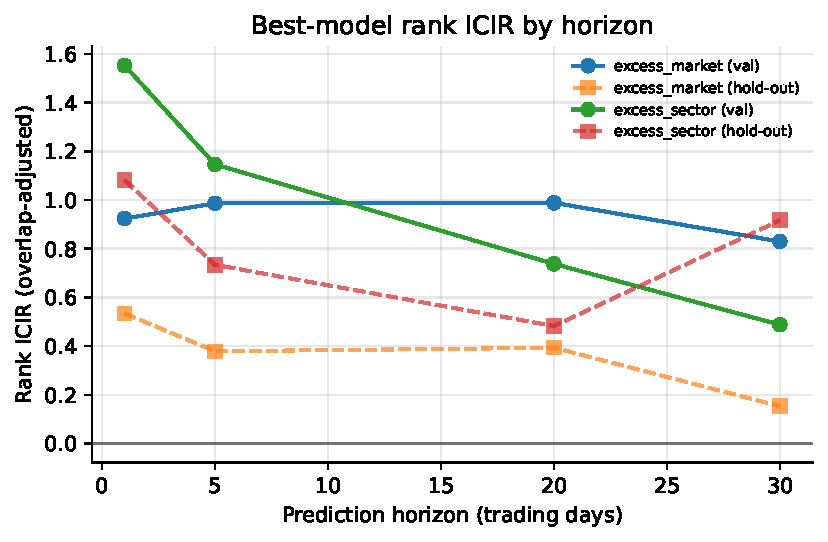
\includegraphics[width=\linewidth]{fig_horizon_icir.pdf}
    \caption{Best-model rank ICIR by horizon (validation vs hold-out), per
    target family.}\label{fig:horizon}
  \end{minipage}\hfill
  \begin{minipage}{0.49\textwidth}\centering
    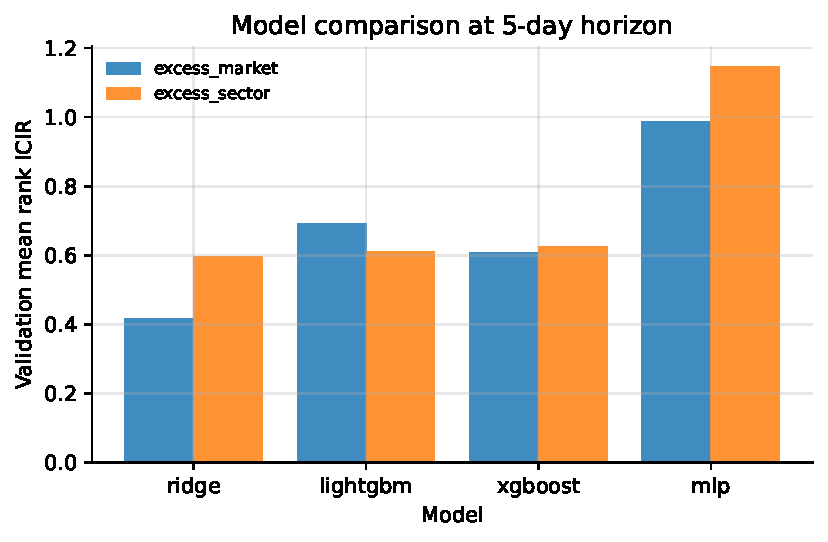
\includegraphics[width=\linewidth]{fig_model_comparison.pdf}
    \caption{Validation mean ICIR by model at the 5-day horizon.}\label{fig:models}
  \end{minipage}
\end{figure}

\textbf{Overlap correction matters.} Fig.~\ref{fig:overlap} contrasts the
overlap-adjusted hold-out ICIR with the naive overlapping value. The naive
metric inflates sharply with horizon (to $\approx$3--10 at 30--90 days) while the
adjusted metric stays modest ($\le 1.3$); reporting the naive number would
manufacture a long-horizon ``signal'' that is pure window overlap. The
Sharpe$>3$/ICIR$>5$ sanity gate flags none of the adjusted runs.

\textbf{Stability across regimes.} Fig.~\ref{fig:stability} shows per-fold ICIR
across the expanding walk-forward. The signal is positive but \emph{variable}
across folds, and the hold-out value (dashed) sits below the validation mean ---
the expected out-of-sample decay. The 90-day horizon is excluded from selection
(too few non-overlapping validation periods for a stable ICIR), and the
longer-horizon hold-out Sharpe values are estimated from few non-overlapping
periods and should be read as noisy. The ensemble search also emits regime
slices whenever a split overlaps the default stress windows (GFC 2008,
COVID-2020, and inflation-2022); with the fixed ensemble split used here, the
available ensemble stress rows are COVID-2020 in validation and inflation-2022 in
test, while 2008 is covered only by the broader walk-forward stability analysis.

\begin{figure}[H]
  \centering
  \begin{minipage}{0.49\textwidth}\centering
    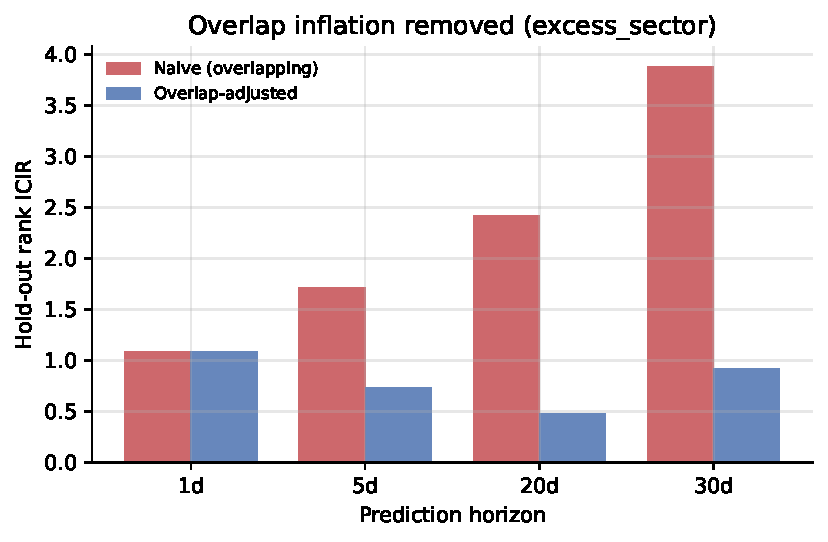
\includegraphics[width=\linewidth]{fig_overlap_adjustment.pdf}
    \caption{Overlap-adjusted vs naive (overlapping) hold-out ICIR by
    horizon.}\label{fig:overlap}
  \end{minipage}\hfill
  \begin{minipage}{0.49\textwidth}\centering
    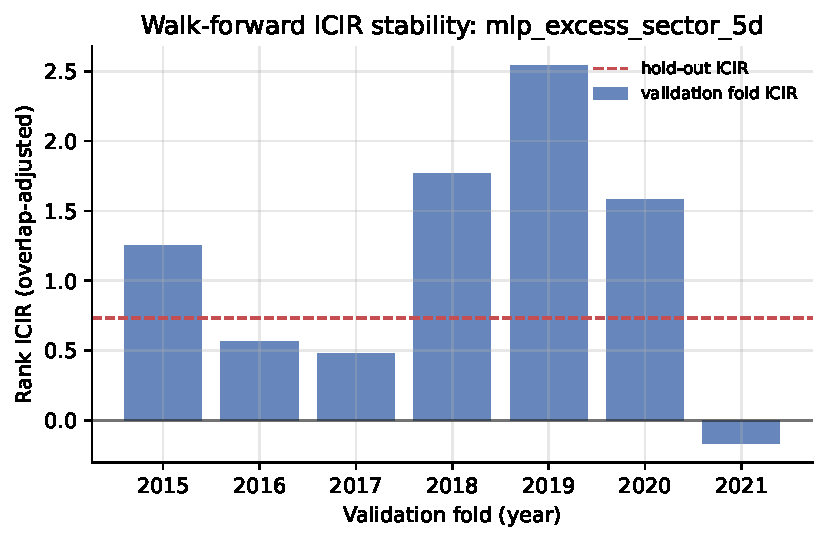
\includegraphics[width=\linewidth]{fig_fold_stability.pdf}
    \caption{Walk-forward per-fold ICIR for the headline run.}\label{fig:stability}
  \end{minipage}
\end{figure}

\textbf{Hold-out performance.} Table~\ref{tab:results} reports the untouched
post-2022 hold-out, net of 5~bps/side cost. The numbers are deliberately modest
and the simple baseline leads: realistic cross-sectional equity ``alpha'' from
price/volume features alone is small, and the trained models' apparent in-sample
edge does not translate into out-of-sample value here.

\begin{table}[t]
  \centering
  \caption{Untouched hold-out (2022--2026), net of 5~bps/side cost. The
  single-factor momentum baseline beats the validation-selected models on IC,
  ICIR, Sharpe, return, \emph{and} turnover. Parenthetical ICIR is the naive
  overlapping value, shown only to document inflation. Best per block in
  \textbf{bold}.}\label{tab:results}
  \small
  \setlength{\tabcolsep}{4pt}
  \begin{tabular}{llccccc}
    \toprule
    Horizon & Config & Rank IC & ICIR (raw) & Net Sharpe & Ann.\ Ret & Turnover \\
    \midrule
    5d  & Momentum baseline (sector)            & \textbf{0.024} & \textbf{1.06} (2.10) & \textbf{1.05} & \textbf{13.5\%} & \textbf{0.16} \\
    5d  & MLP \emph{(val-selected, sector)}      & 0.013 & 0.73 (1.72) & 0.17 & 1.2\% & 0.59 \\
    5d  & Ridge (sector)                        & 0.010 & 0.40 (0.99) & 0.53 & 5.1\% & 0.65 \\
    5d  & LightGBM (sector)                     & 0.009 & 0.20 (1.17) & 0.24 & 1.7\% & 0.53 \\
    \midrule
    20d & Momentum baseline (market)            & \textbf{0.043} & 0.71 (3.62) & \textbf{1.12} & \textbf{13.1\%} & \textbf{0.29} \\
    20d & LightGBM \emph{(val-selected, market)} & 0.028 & 0.39 (2.47) & 0.49 & 5.5\% & 0.64 \\
    20d & Ridge (market)                        & 0.029 & 0.54 (2.27) & 0.76 & 9.8\% & 0.61 \\
    \bottomrule
  \end{tabular}
\end{table}

% ===========================================================================
\section{Discussion}
\label{sec:discussion}
% ===========================================================================

\textbf{Overfitting and the validation--hold-out gap.} The clearest evidence of
overfitting is in the results themselves: models selected on validation ICIR
fail to beat a single momentum factor on the headline 5-day raw rank test, and
the model with the best validation ICIR (the MLP) is not the best economic
hold-out model. The 10-day sector-neutral result is more favorable to tree/graph
models on Sharpe and drawdown, but that is a risk-adjusted win, not a blanket
claim that ML dominates momentum on mean rank IC. We use heavy regularization
(Ridge penalty, tree depth/leaf/subsample limits, MLP dropout + weight decay +
early stopping), select hyperparameters on validation folds only, and report a
single untouched hold-out precisely so this gap is \emph{visible} rather than
hidden, with the Sharpe$>3$/ICIR$>5$ gate catching anything ``too good''.

\textbf{Multiple testing.} The original grid is large enough that the best
Sharpe must be treated as a selected maximum, not as a single pre-specified
experiment. For the 10-day residual overlay, raw hold-out Sharpe is 0.989 and
the probabilistic Sharpe ratio versus zero is essentially one; however, the
bootstrap 95\% Sharpe interval is $[-0.066,2.007]$. After deflating for the
searched configurations, DSR falls to 0.0247 using only same-target trials and
0.00025 using the full grid. CSCV across the overnight strategy matrix gives
PBO $=34.3\%$. This is the most important statistical conclusion: the overlay
is a promising research lead, but not a statistically deflated production alpha.

\textbf{Factor attribution.} The dataset lacks a full commercial risk model and
fundamental value/quality factors, but we can still neutralize the final signal
against available style proxies: liquidity/size
(\texttt{log\_dollar\_volume}), volatility (\texttt{vol\_20d}), beta
(\texttt{beta\_60d}), Amihud illiquidity, short-term reversal
(\texttt{ret\_5d}), and 12--1 momentum. This proxy factor-neutral overlay keeps
some rank information (rank IC $0.021$), but net Sharpe drops from 0.989 to
0.433 and the non-overlapping Fama--MacBeth signal coefficient has
$t=-0.08$. The evidence therefore does not support a claim of independent
style-neutral alpha.

\textbf{Look-ahead leakage.} Addressed structurally: one-day execution lag,
label purge on both sides, horizon embargo, and train-only preprocessing. We
also verified that a no-embargo diagnostic inflates metrics, confirming the
controls bind.

\textbf{Survivorship bias.} The dataset is current-membership-on-history, so
results are optimistically biased and cannot be treated as a production backtest.
The audit adds a numeric sensitivity rather than only a caveat: applying a
delisting overlay of annual delisting rate $\times$ average delisting loss to
the short-side exposure leaves the residual overlay Sharpe at 0.953 in a base
case (2\% annual delisting rate, $-30\%$ average delisting return) and 0.839 in
a stress case (5\%, $-50\%$). This bound is still not a true correction; the
right fix is point-in-time constituents and delisting returns.

\textbf{Foundation models.} Kronos was tested only as a small zero-shot
exploration. On this universe the larger random-date benchmark had negative
2022--2026 test ICs, so it is moved to the ``not yet useful'' bucket rather than
treated as a headline model.

\textbf{Data quality.} Prices are split-adjusted; dividend adjustment is
uncertain and treated as a minor caveat. We winsorize features and filter the
illiquid decile so bad ticks and microcaps do not dominate.

\textbf{Turnover, capacity, and market impact.} We charge 5~bps per side on
realized turnover and rebalance only every $h$ days. Turnover is itself
decisive: the trained models churn $\sim$60\% per rebalance versus
$\sim$16--28\% for the momentum benchmark, and the residual overlay turns over
36.8\%. A simple square-root impact stress test, calibrated to 10~bps at 1\%
ADV participation, gives overlay Sharpe 0.902 at \$100M AUM, 0.794 at \$500M,
and 0.713 at \$1B, with 95th percentile participation rising to 24.5\% at
\$1B. This is not an execution model, but it is enough to show that capacity and
short-side liquidity are first-order constraints.

\textbf{Regime dependence.} Walk-forward folds span 2008, 2020, and 2022 stress
periods; Fig.~\ref{fig:stability} shows the signal is not uniform across
regimes, motivating the market/breadth/dispersion regime features rather than a
single static model.

\textbf{Economic intuition.} The one signal that clearly survives out of sample
is cross-sectional momentum --- a well-documented behavioural underreaction
effect --- which is precisely why the single-factor baseline is so hard to beat.
The multivariate models mostly add estimation variance, not orthogonal signal,
on top of it.

% ===========================================================================
\section{Limitations and Conclusion}
% ===========================================================================

This study delivers an honest, reproducible cross-sectional relative-return
pipeline for the S\&P~500 using only price/volume and light metadata. The key
discipline is methodological: non-overlapping evaluation, walk-forward
selection, explicit leakage controls, and a single-factor baseline that every
model must clear in a clearly specified metric. The realistic conclusion is
sobering: with these features, the trained multivariate and graph models do
\emph{not} pass a production-grade alpha audit. The 5-day and 20-day headline
tests still favor the simpler momentum factor, and the best 10-day residual
overlay is attractive only before multiple-testing deflation and proxy
factor-neutral attribution. I would not trade the current model as a standalone
alpha. The useful output is the triage: keep 12--1 momentum as the benchmark,
treat residual ML as a research lead only, make capacity and turnover part of
selection, and require point-in-time constituents, delisting returns, DSR/PBO,
and style-factor-neutral IC before promoting any future signal to a trading
claim.

\end{document}
